\section{Модификация проекта «Компилятор формул»}
\subsection*{Постановка задачи}
В проекте <<Компилятор формул>> была поставлена задача модифицировать эталонный проект следующим образом: <<В предположении, что язык стекового калькулятора расширен правоассоциативной и имеющей максимальный приоритет операцией \verb|^| возведения в степень, компилировать формулы, содержащие эту операцию>>.


С формальной точки зрения компилятор представляет собой программную реализацию некоторой функции: $\tau\colon L_1 \rightarrow L_2$,  действующей из множества цепочек одного языка $L_1$ в множество цепочек другого $L_2$ таким образом, что $\forall \omega \in L_1$  семантика цепочек $\omega$  и $\tau(\omega) \in L_2$  совпадает.
Нужный нам компилятор представляет собой программную реализацию отображения из множества цепочек языка $L(G_0)$  в множество цепочек языка $L(G_S)$ По этой причине его можно рассматривать, как функцию на пространстве последовательностей~\cite{stack}.

Рассмотрим в качестве входного языка $L(G_0)$ язык правильных арифметических формул, дополненный операцией  возведения в степень, являющейся правоассоциативной и имеющей максимальный приоритет. При этом грамматика $G_0$ вышеуказанного языка будет задаваться следующей НФБН:
\\

\begin{center}
\begin{tabular}{rll}
    $F  \rightarrow$ & $T$  &  $|$ $F+T$ $|$ $ \ F-T $\\
    $T  \rightarrow$ & $M$  &  $|$ $T*M$ $|$ $ \  T/M $\\
    $M  \rightarrow$ & $F$  &  $|$ $M$ \^~$F $   $|$ $ \ V $\\
    $V  \rightarrow$ & $a$  &  $| \ b  \ | \  c \  |  ...  |  \  z $\\ 
\end{tabular} 
\end{center}
Выходным языком будем считать язык $L(G_S)$ стекового калькулятора, грамматика $G_S$ которого также расширена указанной операцией  и задаётся такой НФБН:

\begin{center}
\begin{tabular}{rll}
     $e  \rightarrow \ e e + \ | \ e e - \ | \ e e * \ | \ e e / \ | \ e e$ \^~ $| \ a \ | \ b \ | \ ... \ | \ z \ $ \\
\end{tabular} 
\end{center}
\subsection*{Теоретические аспекты}

Стековый компилятор $\tau$ представляет собой программную реализацию отображения из множества цепочек языка $L(G_0)$ в множество цепочек языка $L(G_S)$. По этой причине его можно рассматривать, как функцию на пространстве последовательностей. Данная функция не является индуктивной, так как результатом компиляции двух произвольных цепочек $w_1 = a-b$ и $w_1 = (a-b)$ является одна и та же цепочка $a \ b \ -$. Если же дописать к обеим цепочкам $x=*c$, результаты компиляции соответствующих цепочек буду выглядеть следующим образом: $a \ b \ c \ * \ - \ $   и  $ \ a \ b \ - \ c \ *$. А это значит, что $\tau(w_1\circ x) \ne \tau(w_2\circ x)$.

Поэтому возникает необходимость построить индуктивное расширение $T$ функции $\tau$ для реализации однопроходного алгоритма. Очевидно, что рекурсивный компилятор формул не подходит для решения данной задачи, а значит, необходимо применить другой алгоритм, основанный на использовании тривиального стека. Для его реализации необходимо определить ряд условий: \\
\begin{itemize}
\item левая скобка \verb|(SYM_LEFT)| не предшествует ничему;
\item правая скобка \verb|(SYM_RIGHT)| предшествует всему;
\item одна арифметическая операция предшествует другой, если её приоритет не ниже, чем у второй;
\item если арифметическая операция является операцией возведения в степень~--- её приоритет выше, чем у какой-либо другой, и операции справа от неё выполняются согласно правилам правой ассоциативности.
\end{itemize} 


Для автоматической обработки конца формулы можно просто взять в скобки всю исходную формулу.

\subsection*{Описание используемых структур и применяемых алгоритмов}

Для решения задачи прежде всего необходимо реализовать тривиальный стек на базе вектора, чтобы размещать в нём отложенные операции. В языке Ruby массив (экземпляр класса Array) имеет все необходимые для этого методы, что только упрощает написание программного кода.
Также введём некоторые константы, задающие тип символа:
\begin{itemize}
\item \verb|SYM_LEFT = 0|  ~---  <<\verb|(|>> 
\item \verb|SYM_RIGHT = 1| ~--- <<\verb|)|>> 
\item \verb|SYM_OPER = 2| ~--- <<\verb|+|>>, <<\verb|-|>>, <<\verb|*|>>, <<\verb|/|>> 
\item \verb|SYM_OTHER = 3| ~---~ добавленная операция ~  \verb|^|
\end{itemize}


Модификация эталонного проекта заключается в повышении приоритета добавленной операции (возведения в степень) по отношению к другим операциям. Для этого в классе \verb|Compf| стекового компилятора, выведенного из уже реализованного класса \verb|Stack|, был изменён метод \verb|priority|:
\begin{lstlisting}
 def priority(c)
    return 3 if (c =='^') 

    (c == '+' or c == '-') ? 1 : 2
 end
\end{lstlisting}
Далее требуется изменить ассоциативность арифметической операции. Для этого необходимо в методе \verb|precedes?|, определяющем отношение предшествования, заменить \verb|>=| на \verb|>|:

\begin{lstlisting}
  def precedes?(a, b)
    return false if sym_type(a) == SYM_LEFT 
    return true  if sym_type(b) == SYM_RIGHT
    if (priority(a)==3 && priority(b)==3)
    priority(a) > priority(b) 
    else
    priority(a) >= priority(b)
    end
  end
\end{lstlisting}

 Многие значительно более сложные задачи на модификацию также сводятся к минимальным изменениям в тексте программы и не требует изменения структуры всей реализации в целом~\cite{stack}.

Ниже представлен снимок экрана, демонстрирующий работу программы: \\ \verb|compf.rb|:
\begin{figure}[ht!]
\begin{center}
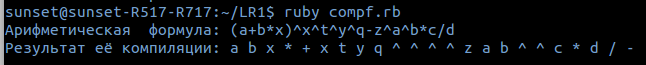
\includegraphics[width=1\hsize]{images/screen}
\end{center}
\caption{Вывод программы}\label{fig:screen}
\end{figure}


